% !TeX document-id = {c68ea1ac-ebac-4541-a297-17005c6d2297}
% !TeX encoding = UTF-8
% !TeX spellcheck = en_US
% !TeX TS-program = pdflatex
% !TeX TXS-program:bibliography = biber -l zh__pinyin --output-safechars %

\documentclass[12pt]{article}

% to be `\input` in subfolders,
% ... therefore the path should be relative to subfolders.

\usepackage{iftex}
\ifPDFTeX
\else
	\usepackage[UTF8
		,heading=false
		,scheme=plain % English Document
	]{ctex}
\fi
%\ctexset{autoindent=true}
\usepackage{indentfirst}

\input{../.modules/basics/macros.tex}
\input{../.modules/preamble_base.tex}
%\input{../.modules/preamble_notes.tex}
\input{../.modules/basics/biblatex.tex}


%Misc
%	\usepackage{lilyglyphs}
%	\newcommand{\indicator}{$\text{\clefG}$}
%	\newcommand{\indicatorInline}{$\text{\clefGInline}$}

\usepackage{titling}
\setlength{\droptitle}{-2.5\baselineskip}



% Settings
\counterwithout{equation}{section}
\mathtoolsset{showonlyrefs=false}
%\DeclareTextFontCommand{\textbf}{\sffamily}

% Spacing
\usepackage[
	papersize={200mm,150mm},
	hmargin=1.5cm,
	vmargin={1.5cm,1.7cm}
]{geometry}
\geometry{footnotesep=2\baselineskip} % pre footnote split
\setlength{\parskip}{.5\baselineskip}
\renewcommand{\baselinestretch}{1.15}

\usepackage{ragged2e}


%% List
%	\setlist*{
%		listparindent=\parindent
%		,labelindent=\parindent
%		,parsep=\parskip
%		,itemsep=1.2\parskip
%	}


\usepackage{tikz}
\usepackage{caption}
%\usepackage{snapshot}

\renewenvironment{frame}[1]%
	{\section*{#1}}%
	{\clearpage}

\usepackage{enumitem}

\setlength{\parindent}{0pt}
\setlength{\droptitle}{-7.5\baselineskip}
\pretitle{%
	\bfseries\noindent\large\\[2ex]
	\arxiv{2303.04836}
	\Large\\
}
\title{Glue-on AdS holography for $T\bar T$-deformed CFTs}
\posttitle{%
	\par%\vspace{.5\baselineskip}
	\vspace{-.7\baselineskip}
	\noindent\rule{\linewidth}{1.2pt}\par
	\vspace{0.\baselineskip}
}

\preauthor{\noindent}
\author{%
	Luis Apolo,
	Peng-Xiang Hao \textkai{郝鹏翔},
	\textbf{Wen-Xin Lai \textkai{赖文昕}},
	and Wei Song \textkai{宋伟}
}
\postauthor{\vspace{-3.8\baselineskip}}
\date{}


\addbibresource{glueon-beamer.bib}

\usepackage{xspace}
\newcommand{\TTbar}{\texorpdfstring{\ensuremath{T\bar{T}}}{TTbar}\xspace}

\begin{document}

\maketitle
\thispagestyle{empty}

\begin{equation*}
\large
\hspace{-2em}
\begin{aligned}
	\textbf{Proposal:}\ \,
	\textrm{Cutoff}
	\ &/\ %
	\text{\textbf{\textit{glue-on}} $\mrm{AdS}_3$ Gravity}
	\!\!&\equiv\ %
	\textrm{\TTbar deformed $\mrm{CFT}_2$} \\[.5ex]
	\mu < 0
	\ &/\ %
	\mu > 0
	&
\end{aligned}
\end{equation*}

\vspace{-1ex}
\hspace{-1em}
\begin{minipage}{.57\linewidth}
\centering
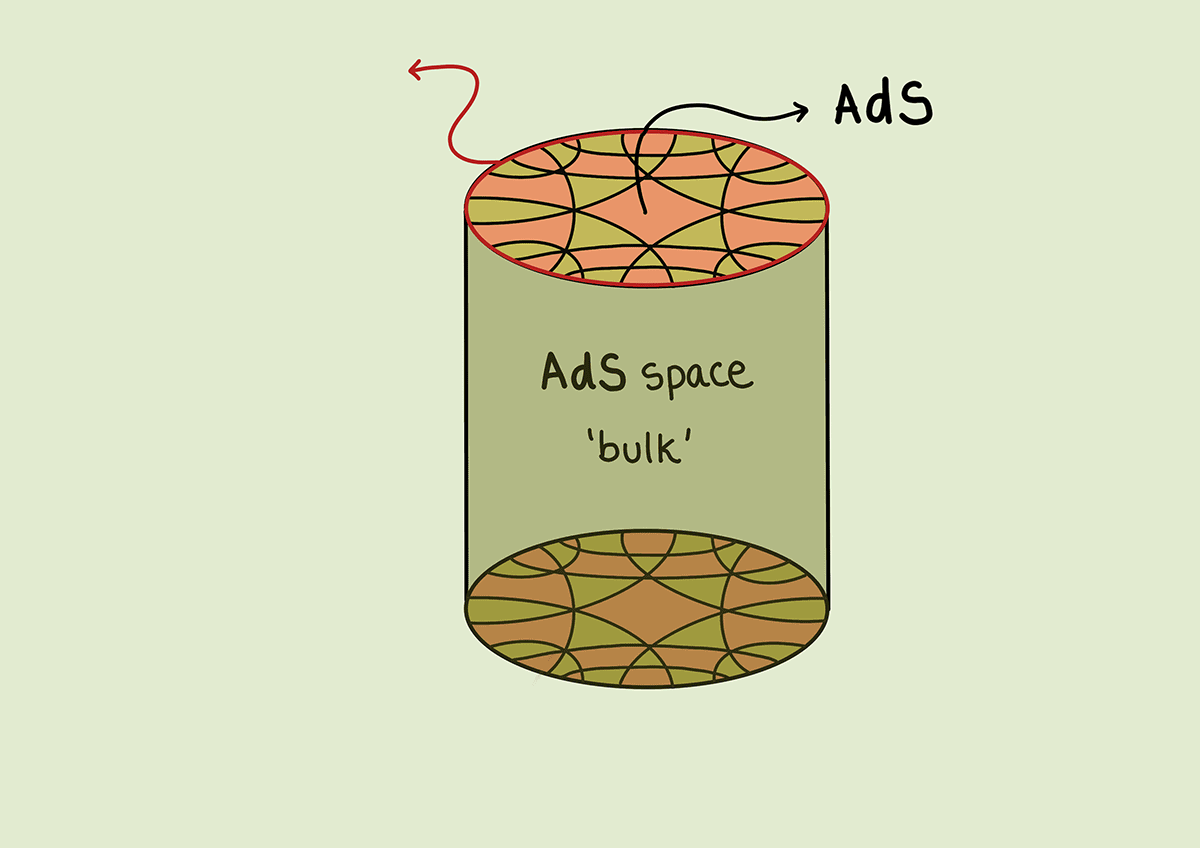
\includegraphics[width=\linewidth]{img/ads-cft-cutoff.png}

\vspace{-.3\baselineskip}
\scriptsize\hspace{-2.5em}
Image courtesy: \textsl{\citeauthor{AldegundePWSep22}, 2022}
\end{minipage}%
\begin{minipage}{.43\linewidth}
\vspace{-6ex}
\begin{itemize}[leftmargin=-3em,itemsep=-.5ex]
\item \TTbar: $ \dfrac{\pd I}{\pd\mu} = {8 \pi} \displaystyle\int d^2x \, T\bar T$\\[1ex]
well-defined for $\mu \in \mbb{R}$
\item $\mrm{AdS}_3^{\sidenote{*}}$: extended beyond infinity!\\
We try to make sense of the \textit{\textbf{``glue-on''}}:

\begin{itemize}[leftmargin=5.5em,noitemsep]
\item Spectrum: $E(\mu)$, $J(\mu)$
\item Flow equations for $\ave{\tr T}$
\item Bounds from geometry (horizons)
\item ...
\end{itemize}

\item Extended Ryu-Takayanagi / HRT\\
	$\leadsto$ \textit{\TTbar deformed entanglement?}
	at \sidenote{\large\textbf{Y306}}
\end{itemize}



%\hfill
%\mbox{
%	
\includegraphics[width=3.5em]{img/inspire-qr-cy.png}
%	\hspace{-3.2em}
%}

\end{minipage}

\clearpage
\end{document}
